\documentclass{article}
\usepackage{graphicx} % Required for inserting images
\usepackage[utf8]{inputenc}
\usepackage{hyperref}
\usepackage[catalan]{babel}
\usepackage{pgfplots}
\pgfplotsset{compat=1.18}
\usepackage{float}
\usepackage{amsmath}
\usepackage{parskip}
\usepackage{listings}
\usepackage{multirow}
\usepackage{url}

\newtheorem{defibox}{Definició}[section] % Numerat per seccions

\lstset{
    language=C,
    basicstyle=\ttfamily\small,
    keywordstyle=\color{blue}\bfseries,
    commentstyle=\color{gray}\itshape,
    stringstyle=\color{red},
    showstringspaces=false,
    breaklines=true,
    frame=none,
    tabsize=4,
    numbers=left,
    numberstyle=\tiny\color{gray}
}

\hypersetup{
    colorlinks=true,
    linkcolor=black,
    filecolor=magenta,
    urlcolor=blue,
    citecolor=green
}

\title{Pràctica OpenMP \\ Computació d'Altes Prestacions}
\author{Miguel Arlindo Correia Salgueiro - 1747746 \\Oriol Figueras Ollé - 1748144}
\date{}

\begin{document}

\maketitle

\newpage
\tableofcontents
\newpage

\section{Introducció}

L'objectiu principal d'aquesta pràctica consisteix en paral·lelitzar una implementació escrita en $C$ d'una xarxa neuronal de tipus perceptró fent servir una aproximació de paral·lelització multi-core. S'usa OpenMP per fer l'implementació.

S'usa també Git com a eina de control de versions.

\subsection{Compilació i execució}

Per a compilar aquest projecte s'ha creat un \textit{makefile} per fer la compilació més senzilla.
En el \textit{makefile} hi ha definides dues maneres de compilar, una amb la paral·lelització implementada i l'altra de manera seqüencial.
A continuació es mostra el contingut del fitxer:
\begin{verbatim}
CC     := gcc
OPT    := -Ofast
LDLIBS := -lm

SRC := main.c \
       common/common.c \
       configuration/config.c \
       layer/layer.c \
       randomizer/randomizer.c \
       initialize/initialize.c \
       training/training.c

HDR := $(wildcard *.h */*.h)

.PHONY: all seq par clean

all: seq par
seq: exec_seq
par: exec_par

exec_seq: $(SRC) $(HDR)
        $(CC) $(OPT) $(SRC) -o $@ $(LDLIBS)

exec_par: $(SRC) $(HDR)
        $(CC) $(OPT) -fopenmp $(SRC) -o $@ $(LDLIBS)

clean:
        rm -f exec_seq exec_par

\end{verbatim}

D'aquesta manera, amb un simple \texttt{make seq} o \texttt{make par} ja es crea l'executable corresponent, amb els noms de \texttt{exec\_seq} i \texttt{exec\_par} respectivament. També es pot usar \texttt{make all} per generar tots dos executables. Per executar el programa simplement cal fer \texttt{./exec\_seq} o \texttt{./exec\_par}. 

Es poden eliminar els executables també usant el \textit{makefile}, amb \texttt{make clean}.

Per a fer útil el \textit{makefile} creat, s'ha modificat el \textit{seq.sub} donat i s'ha creat un \textit{par.sub} addicional.

El fitxer \textit{seq.sub} és el següent:
\begin{verbatim}
#!/bin/bash
#SBATCH -N 1 # number of nodes
#SBATCH --exclusive 
#SBATCH --partition=nodo.q

module add gcc/13.2.1

make seq

## perf stat ./exec_seq configuration/configfile.txt
./exec_seq configuration/configfile.txt
\end{verbatim}

I el fitxer \textit{par.sub} està construït de manera similar, amb la lògica addicional de poder passar el nombre de threads com a argument del \textit{sbatch}:
\begin{verbatim}
#!/bin/bash
#SBATCH -N 1 # number of nodes
#SBATCH --exclusive 
#SBATCH --partition=nodo.q

THREADS=${1:-4} # default number of threads is 4

module add gcc/13.2.1

make par

export OMP_NUM_THREADS=$THREADS
echo "Threads: $OMP_NUM_THREADS"

## perf stat ./exec_par configuration/configfile.txt
./exec_par configuration/configfile.txt
\end{verbatim}

\noindent Cal destacar que les ordres exactes per tal de enviar les execucions, són:

\begin{verbatim}
# Seqüencial
sbatch seq.sub

# Paral·lel amb n threads
sbatch par.sub n
\end{verbatim}

\newpage
\section{Estratègia de paral·lelització}

L'estratègia de paral·lelització usada en aquesta pràctica és una paral·lelització basada en bucles. 
S'ha escollit aquesta estratègia per la quantitat de \textit{for} que hi ha en el \textit{training.c} i per la dificultat afegida de la paral·lelització basada en tasques, que implicaria una modificació substancial del codi base.

\subsection{Paral·lelització de \textit{feed\_input()}}

Aquesta funció es pot paral·lelitzar, ja que les operacions dins el bucle de la funció són independents les unes de les altre.
Tot i això, pot no suposar un gran avantatge, perquè cada crida d'aquesta funció només requereix fer una copia de 1024 valors del patró d'entrada i la sobrecàrrega de crear i sincronitzar threads pot ser superior al temps estalviat al paral·lelitzar.

La funció paral·lelitzada és:
\begin{lstlisting}
void feed_input(int i) {
    #pragma omp parallel for
    for (int j = 0; j < num_neurons[0]; j++)
        lay[0].actv[j] = input[i][j];
}
\end{lstlisting}

A continuació es mostren unes taules comparatives del temps d'execució del programa amb únicament la funció \textit{feed\_input()} paral·lelitzada, amb diversos nombres de threads.

\begin{table}[H]
    \centering
    \begin{tabular}{|c|c|c|}
        \hline
        \textbf{Execució seqüencial} & \textbf{Execució paral·lela 1} & \textbf{Execució paral·lela 2} \\ \hline
        40,5441 s & 41,4919 s & 42,0177 s \\ \hline
        \textbf{Execució paral·lela 3} & \textbf{Execució paral·lela 4} & \textbf{Execució paral·lela 5} \\ \hline
        41,8789 s & 43,8571 s & 44,0709 s \\ \hline
    \end{tabular}
    \caption{Taula comparativa de temps de programa amb \textit{feed\_input()} paral·lelitzat amb 4 threads.}
    \label{tab:f1_4trheads}
\end{table}

\begin{table}[H]
    \centering
    \begin{tabular}{|c|c|c|}
        \hline
        \textbf{Execució seqüencial} & \textbf{Execució paral·lela 1} & \textbf{Execució paral·lela 2} \\ \hline
        40,5441 s & 42,0085 s & 42,3634 s \\ \hline
        \textbf{Execució paral·lela 3} & \textbf{Execució paral·lela 4} & \textbf{Execució paral·lela 5} \\ \hline
        44,7099 s & 44,0000 s & 42,2120 s \\ \hline
    \end{tabular}
    \caption{Taula comparativa de temps de programa amb \textit{feed\_input()} paral·lelitzat amb 8 threads.}
    \label{tab:f1_8trheads}
\end{table}

\begin{table}[H]
    \centering
    \begin{tabular}{|c|c|c|}
        \hline
        \textbf{Execució seqüencial} & \textbf{Execució paral·lela 1} & \textbf{Execució paral·lela 2} \\ \hline
        40,5441 s & 42,9662 s & 42,7769 s \\ \hline
        \textbf{Execució paral·lela 3} & \textbf{Execució paral·lela 4} & \textbf{Execució paral·lela 5} \\ \hline
        45,3571 s & 46,3817 s & 43,7859 s \\ \hline
    \end{tabular}
    \caption{Taula comparativa de temps de programa amb \textit{feed\_input()} paral·lelitzat amb 12 threads.}
    \label{tab:f1_12trheads}
\end{table}

Com es pot observar a les taules, paral·lelitzar aquesta funció no aporta un benefici, de fet perjudica el programa i el fa més lent perquè es tarda més a crear tots els threads i dividir la càrrega de treball que en executar el treball.

Per aquest motiu, no s'aplicarà la paral·lelització a aquesta funció inicialment, però es considerarà afegir la paral·lelització a nivell global, per veure si combinar aquesta paral·lelització amb la paral·lelització d'altres funcions pot ser útil en la secció \texttt{\nameref{sec:performance_analysis}}.

\subsection{Paral·lelització de \textit{init\_deltas()}}

Aquesta és una funció que presenta diversos bucles paral·lelitzables, tot i que cal tenir en compte alguns matisos.

El primer \textit{for} es pot paral·lelitzar, però no resulta convenient fer-ho directament amb \textbf{\texttt{\#pragma omp parallel for}}. El motiu és que, si per exemple utilitzem 4 threads i paral·lelitzem el primer \textit{for}, repartirem les 4 iteracions del bucle entre els 4 threads. Aquesta distribució pot ser perjudicial per al temps d'execució, ja que cada iteració del bucle exterior executa dos bucles interiors amb una càrrega de treball diferent.

Per exemple, en el segon bucle interior, quan
\texttt{i = 0}, es realitzen
\[
1024 \cdot 500 = 512000
\]
assignacions, mentre que en l'última iteració,
quan \texttt{i = 3}, només es realitzen
\[
135 \cdot 10 = 1350
\]
assignacions.
Això provocaria un repartiment molt desequilibrat del treball,
ja que alguns threads acabarien molt abans que altres i
haurien d'esperar que finalitzés el thread amb més càrrega.

Per aquest motiu, utilitzem \textbf{\texttt{\#pragma omp parallel}} per crear una única regió paral·lela en la qual es manté el mateix equip de threads durant l'execució dels diferents bucles.
D'aquesta manera, evitem crear diverses regions paral·leles independents. Si paral·lelitzéssim per separat els dos bucles interiors amb \textbf{\texttt{\#pragma omp parallel for}},
tindríem 8 regions paral·leles en total, ja que el bucle exterior té 4 iteracions i dins de cadascuna hi ha 2 bucles paral·lelitzats.
Això introduiria una sobrecàrrega addicional associada a l'entrada i sortida de les regions paral·leles.

Pel que fa als bucles interiors, en el primer utilitzem \textbf{\texttt{\#pragma omp for nowait}}.
Aquest bucle realitza assignacions sobre el vector \texttt{dbias}, amb un nombre d'iteracions que va des de 1024 en la primera capa fins a 135 en l'última iteració del bucle exterior.

Amb \textbf{\texttt{\#pragma omp for}} aconseguim repartir les iteracions del bucle entre els threads de la regió paral·lela. A més, amb la clàusula \textbf{\texttt{nowait}} eliminem la barrera de sincronització implícita que hi ha al final del bucle. D'aquesta manera, quan un thread acaba les iteracions que té assignades, pot continuar cap al següent bucle sense haver d'esperar que els altres threads acabin.

Això és possible perquè els dos bucles són independents: el primer inicialitza el vector \texttt{dbias}, mentre que el segon inicialitza el vector \texttt{dw}. Per tant, no existeixen dependències de dades entre aquestes dues operacions.
Amb aquesta modificació podem reduir part del temps dedicat a la sincronització.

De totes maneres, com que les operacions del primer bucle són simplement assignacions a zero, totes les iteracions tenen pràcticament el mateix cost computacional. Per aquest motiu, és probable que els threads acabin les seves iteracions en temps semblants i que la millora obtinguda amb \textbf{\texttt{nowait}} sigui petita.

D'altra banda, en el segon bucle interior utilitzem \textbf{\texttt{\#pragma omp for schedule(static)}}. Aquest és el bucle amb més càrrega de treball, especialment en la primera iteració del bucle exterior, on es realitzen 512000 assignacions.

Hem escollit \textbf{\texttt{schedule(static)}} perquè totes les iteracions tenen pràcticament el mateix cost computacional. D'aquesta manera, OpenMP reparteix les iteracions de forma estàtica i equilibrada entre els threads, sense necessitat d'assignar nous blocs de treball dinàmicament.
Això permet reduir la sobrecàrrega associada a la planificació de les iteracions.

El codi paral·lelitzat és el següent:

\begin{lstlisting}
void init_deltas() {
    #pragma omp parallel
    {
        for (int i = 0; i < num_layers - 1; i++) {

            #pragma omp for nowait
            for (int j = 0; j < num_neurons[i]; j++)
                lay[i].dbias[j] = 0.0;

            #pragma omp for schedule(static)
            for (int j = 0; j < num_neurons[i + 1] * num_neurons[i]; j++)
                lay[i].dw[j] = 0.0;
        }
    }
}
\end{lstlisting}

A continuació es mostren unes taules comparatives del temps d'execució del programa amb únicament la funció \textit{init\_deltas()} paral·lelitzada, amb diversos nombres de threads.

\begin{table}[H]
    \centering
    \begin{tabular}{|c|c|c|}
        \hline
        \textbf{Execució seqüencial} & \textbf{Execució paral·lela 1} & \textbf{Execució paral·lela 2} \\ \hline
        40.7261 s & 41.0380 s & 40.7334 s \\ \hline
        \textbf{Execució paral·lela 3} & \textbf{Execució paral·lela 4} & \textbf{Execució paral·lela 5} \\ \hline
        42.4691 s & 42.4647 s & 40.7182 s \\ \hline
    \end{tabular}
    \caption{Taula comparativa de temps de programa amb \textit{init\_deltas()} paral·lelitzat amb 4 threads.}
    \label{tab:f2_4trheads}
\end{table}

\begin{table}[H]
    \centering
    \begin{tabular}{|c|c|c|}
        \hline
        \textbf{Execució seqüencial} & \textbf{Execució paral·lela 1} & \textbf{Execució paral·lela 2} \\ \hline
        40.7261 s & 40.7826 s & 42.5414 s \\ \hline
        \textbf{Execució paral·lela 3} & \textbf{Execució paral·lela 4} & \textbf{Execució paral·lela 5} \\ \hline
        43.0108 s & 40.7396 s & 40.8045 s \\ \hline
    \end{tabular}
    \caption{Taula comparativa de temps de programa amb \textit{init\_deltas()} paral·lelitzat amb 8 threads.}
    \label{tab:f2_8trheads}
\end{table}

\begin{table}[H]
    \centering
    \begin{tabular}{|c|c|c|}
        \hline
        \textbf{Execució seqüencial} & \textbf{Execució paral·lela 1} & \textbf{Execució paral·lela 2} \\ \hline
        40.7261 s & 40.8568 s & 40.8120 s \\ \hline
        \textbf{Execució paral·lela 3} & \textbf{Execució paral·lela 4} & \textbf{Execució paral·lela 5} \\ \hline
        43.2060 s & 42.6350 s & 40.8100 s \\ \hline
    \end{tabular}
    \caption{Taula comparativa de temps de programa amb \textit{init\_deltas()} paral·lelitzat amb 12 threads.}
    \label{tab:f2_12trheads}
\end{table}

Com  es veu en les taules, no hem aconseguit una millora de rendiment respecte de l'execució seqüencial.

Una possible explicació és que aquests bucles únicament realitzen assignacions del valor zero als elements dels vectors, de manera que cada iteració té un cost computacional molt reduït. En aquestes condicions, la sobrecàrrega associada a la gestió dels threads, al repartiment del treball i a les sincronitzacions pot superar el temps estalviat gràcies a la paral·lelització.
A més, el rendiment també pot estar limitat per la velocitat d'accés i escriptura a memòria.

Per tant, en aquest cas, paral·lelitzar els bucles no garanteix una reducció del temps d'execució, i els resultats experimentals indiquen que la versió seqüencial resulta més eficient. De totes  maneres, comprovarem si combinar aquesta paral·lelització amb la paral·lelització d'altres funcions pot ser útil en la secció \texttt{\nameref{sec:performance_analysis}}.

\subsection{Paral·lelització de \textit{forward\_prop()}}

En aquesta funció, dels tres bucles, un és paral·lelitzable, un requereix consideracions addicionals i un presenta dependències entre iteracions

El \textit{for} d'índex $i$ no és paral·lelitzable, ja que una iteració usa les dades de la iteració anterior, és a dir hi ha una dependència clara entre iteracions del bucle. Aquesta dependència es fa explícita dins el \textit{for} d'índex $k$, on s'usa \texttt{lay[i-1].actv[k]}.

El \textit{for} d'índex $j$ és paral·lelitzable perquè una iteració és completament independent de la següent i de l'anterior. 

El \textit{for} d'índex $k$ és paral·lelitzable amb un matís, seria possible sempre que es controli l'accés a la variable \texttt{lay[i].z[j]} de manera correcta. Això es podria fer amb un \textbf{\texttt{critical}} o un \textbf{\texttt{atomic}}, però causaria un possible empitjorament del rendiment, ja que els threads estarien tota l'estona esperant per entrar a la regió crítica.

La manera més correcta és usar \textbf{\texttt{reduction}}, però a cada thread li correspondria una càrrega de treball molt petita (un producte i una suma), per la qual cosa suposem que la paral·lelització niuada seria contraproduent.

Per aquest motiu, inicialment es descarta paral·lelitzar aquest bucle, però es revisarà en l'apartat \texttt{\nameref{sec:performance_analysis}} per assegurar la nostra suposició.

La funció paral·lelitzada al bucle d'índex $j$ queda de la següent manera:
\begin{lstlisting}
void forward_prop() {
    #pragma omp parallel
    for (int i = 1; i < num_layers; i++) {
        if (debug == 1) printf("Valors activacio capa %d \n", i);
        #pragma omp for schedule(static)
        for (int j = 0; j < num_neurons[i]; j++) {
            lay[i].z[j] = lay[i].bias[j];
            for (int k = 0; k < num_neurons[i - 1]; k++)
                lay[i].z[j] +=
                    ((lay[i - 1].out_weights[j * num_neurons[i - 1] + k]) *
                     (lay[i - 1].actv[k]));
            if (i < num_layers - 1)  // Relu Activation Function for Hidden Layers
                lay[i].actv[j] = ((lay[i].z[j]) < 0) ? 0 : lay[i].z[j];
            else  // Sigmoid Activation Function for Output Layer
                lay[i].actv[j] = 1 / (1 + exp(-lay[i].z[j]));
            if (debug == 1) printf("%f %f ", lay[i].actv[j], lay[i].z[j]);
        }
        if (debug == 1) printf("\n\n");
    }
}
\end{lstlisting}

S'ha usat el \textbf{\texttt{schedule(static)}} per obtenir un baseline, ja que és la política estàndard d'OpenMP. Es consideraran altres polítiques en la part d'\texttt{\nameref{sec:performance_analysis}}.

A continuació es mostren unes taules comparatives del temps d'execució del programa amb únicament la funció \textit{forward\_prop()} paral·lelitzada, amb diversos nombres de threads.

\begin{table}[H]
    \centering
    \begin{tabular}{|c|c|c|}
        \hline
        \textbf{Execució seqüencial} & \textbf{Execució paral·lela 1} & \textbf{Execució paral·lela 2} \\ \hline
        40,6889 s & 26,3509 s & 26,3722 s\\ \hline
        \textbf{Execució paral·lela 3} & \textbf{Execució paral·lela 4} & \textbf{Execució paral·lela 5} \\ \hline
        26,3609 s & 26,7797 s & 28,2628 s \\ \hline
    \end{tabular}
    \caption{Taula comparativa de temps de programa amb \textit{forward\_prop()} paral·lelitzat amb 4 threads.}
    \label{tab:f3_4trheads}
\end{table}

\begin{table}[H]
    \centering
    \begin{tabular}{|c|c|c|}
        \hline
        \textbf{Execució seqüencial} & \textbf{Execució paral·lela 1} & \textbf{Execució paral·lela 2} \\ \hline
        40,6889 s & 23,4829 s & 23,3459 s \\ \hline
        \textbf{Execució paral·lela 3} & \textbf{Execució paral·lela 4} & \textbf{Execució paral·lela 5} \\ \hline
        23,4431 s & 24,5725 s & 23,5300 s \\ \hline
    \end{tabular}
    \caption{Taula comparativa de temps de programa amb \textit{forward\_prop()} paral·lelitzat amb 8 threads.}
    \label{tab:f3_8trheads}
\end{table}

\begin{table}[H]
    \centering
    \begin{tabular}{|c|c|c|}
        \hline
        \textbf{Execució seqüencial} & \textbf{Execució paral·lela 1} & \textbf{Execució paral·lela 2} \\ \hline
        40,6889 s & 22,9876 s & 23,0159 s \\ \hline
        \textbf{Execució paral·lela 3} & \textbf{Execució paral·lela 4} & \textbf{Execució paral·lela 5} \\ \hline
        24,1328 s & 23,9703 s & 26,8209 s\\ \hline
    \end{tabular}
    \caption{Taula comparativa de temps de programa amb \textit{forward\_prop()} paral·lelitzat amb 12 threads.}
    \label{tab:f3_12trheads}
\end{table}

Els temps d'execució del programa han millorat considerablement. Aparentment, la paral·lelització d'aquesta funció afecta positivament, falta, però acabar d'ajustar el nombre de threads ideal, si val la pena paral·lelitzar el bucle d'índex $k$, i també seria interessant considerar altres polítiques de divisió de càrrega de treball.

Addicionalment, considerar si posar un llindar mínim al nombre de neurones per tal de paral·lelitzar pot ser una idea que valgui la pena explorar.

En conclusió, aquesta funció sí que es paral·lelitza. Es pren com a base la paral·lelització descrita en aquest apartat i s'analitzaran els ítems esmentats a l'apartat d'\texttt{\nameref{sec:performance_analysis}}.

\subsection{Paral·lelització de \textit{compute\_loss()}}

Aquesta és una funció que conté un únic bucle. Per paral·lelitzar-la utilitzarem la directiva \textbf{\texttt{\#pragma omp parallel for private(p) reduction(+:tmpcost) schedule(static)}}.

Aquesta directiva ens permet realitzar diverses operacions. En primer lloc, tenim un \textit{for} de 10 iteracions. Per paral·lelitzar-lo, utilitzem \textbf{\texttt{\#pragma omp parallel for}}, que s'encarrega de distribuir les iteracions del bucle entre els diferents threads disponibles.

D'altra banda, necessitem la clàusula \textbf{\texttt{private(p)}}, ja que \texttt{p} és una variable declarada fora del bucle que, per defecte, seria compartida entre tots els threads. Com que en cada iteració se li assigna un valor diferent, si no utilitzéssim  \textbf{\texttt{private(p)}}, podria passar que diversos threads modifiquessin simultàniament la mateixa variable, provocant una condició de carrera (\textit{race condition}) i, en conseqüència, resultats incorrectes. Amb aquesta clàusula, cada thread disposa de la seva pròpia còpia de la variable \texttt{p}, evitant així possibles conflictes.

Seguidament, la clàusula \textbf{\texttt{reduction(+:tmpcost)}} és essencial en aquesta paral·lelització. Això és degut al fet que \texttt{tmpcost} és una variable que acumula els resultats de les diferents iteracions mitjançant una suma. Si diversos threads modifiquessin aquesta variable simultàniament sense cap mecanisme de protecció, es podrien perdre  actualitzacions i obtenir un resultat incorrecte.

Amb \textbf{\texttt{reduction(+:tmpcost)}}, aconseguim que cada thread disposi d'una còpia privada de \texttt{tmpcost}, inicialitzada a zero, en la qual acumula els resultats de les iteracions que té assignades. Un cop finalitzat el bucle, OpenMP combina totes aquestes sumes parcials per obtenir el valor final de \texttt{tmpcost}. D'aquesta manera, evitem les condicions de carrera i garantim que es tinguin en compte les contribucions de totes les iteracions.

Finalment, hem utilitzat \textbf{\texttt{schedule(static)}} per distribuir les iteracions del bucle de manera estàtica i equilibrada entre els threads. Hem escollit aquesta opció en lloc de
\textbf{\texttt{schedule(dynamic)}} perquè totes les iteracions realitzen pràcticament les mateixes operacions i, per tant, tenen un cost computacional similar. D'aquesta manera, no és necessari realitzar un repartiment dinàmic del treball, que introduiria una sobrecàrrega addicional.

A més, encara que totes les iteracions tenen un cost computacional similar, la funció només realitza 10 iteracions per crida. Per tant, és possible que la sobrecàrrega associada a la gestió de la regió paral·lela, al repartiment del treball i a la reducció dels resultats parcials sigui superior al temps estalviat gràcies a la paral·lelització.

Per aquest motiu, és probable que aquesta paral·lelització no proporcioni una millora significativa del temps d'execució i que, fins i tot, pugui empitjorar el rendiment respecte de la versió seqüencial.

\begin{lstlisting}
float compute_loss(int i) {
    double tmpcost = 0, p;

    #pragma omp parallel for private(p) reduction(+:tmpcost) schedule(static)
    for (int j = 0; j < num_neurons[num_layers - 1]; j++) {
        p = lay[num_layers - 1].actv[j];

        if (lay[num_layers - 1].actv[j] < EPSILON)
            p = EPSILON;
        else if (lay[num_layers - 1].actv[j] > 1 - EPSILON)
            p = 1 - EPSILON;

        tmpcost += desired_outputs[i][j] * log(p)
                 + (1 - desired_outputs[i][j]) * log(1.0 - p);
    }

    return -tmpcost / num_neurons[num_layers - 1];
}
\end{lstlisting}

A continuació es mostren unes taules comparatives del temps d'execució del programa amb únicament la funció \textit{compute\_loss()} paral·lelitzada, amb diversos nombres de threads.

\begin{table}[H]
    \centering
    \begin{tabular}{|c|c|c|}
        \hline
        \textbf{Execució seqüencial} & \textbf{Execució paral·lela 1} & \textbf{Execució paral·lela 2} \\ \hline
        40.6208 s & 41.1932 s & 41.5916 s \\ \hline
        \textbf{Execució paral·lela 3} & \textbf{Execució paral·lela 4} & \textbf{Execució paral·lela 5} \\ \hline
        44.0686 s & 43.5493 s & 41.2481 s \\ \hline
    \end{tabular}
    \caption{Taula comparativa de temps de programa amb textit{compute\_loss()} paral·lelitzat amb 4 threads.}
    \label{tab:f4_4trheads}
\end{table}

\begin{table}[H]
    \centering
    \begin{tabular}{|c|c|c|}
        \hline
        \textbf{Execució seqüencial} & \textbf{Execució paral·lela 1} & \textbf{Execució paral·lela 2} \\ \hline
        40.6208 s & 42.0004 s & 41.9586 s \\ \hline
        \textbf{Execució paral·lela 3} & \textbf{Execució paral·lela 4} & \textbf{Execució paral·lela 5} \\ \hline
        44.4558 s & 44.3085 s & 41.8578 s \\ \hline
    \end{tabular}
    \caption{Taula comparativa de temps de programa amb \textit{compute\_loss()} paral·lelitzat amb 8 threads.}
    \label{tab:f4_8trheads}
\end{table}

\begin{table}[H]
    \centering
    \begin{tabular}{|c|c|c|}
        \hline
        \textbf{Execució seqüencial} & \textbf{Execució paral·lela 1} & \textbf{Execució paral·lela 2} \\ \hline
        40.6208 s & 42.7304 s & 42.8249 s \\ \hline
        \textbf{Execució paral·lela 3} & \textbf{Execució paral·lela 4} & \textbf{Execució paral·lela 5} \\ \hline
        45.1416 s & 44.8602 s & 43.2013 s \\ \hline
    \end{tabular}
    \caption{Taula comparativa de temps de programa amb  \textit{compute\_loss()} paral·lelitzat amb 12 threads.}
    \label{tab:f4_12trheads}
\end{table}

Es pot observar com el rendiment empitjora i, en alguns casos, considerablement. Aquests resultats indiquen que la sobrecàrrega associada a la gestió de les regions paral·leles, al repartiment del treball i a la reducció dels resultats parcials pot superar el temps estalviat gràcies a la paral·lelització. Això provoca que el temps d'execució sigui superior al de la versió seqüencial i ens permet concloure que aquesta paral·lelització, per si sola, no resulta beneficiosa.

De totes maneres, abans de prendre una decisió definitiva, comprovarem si, en combinar aquesta funció amb altres funcions paral·lelitzades, el rendiment global del programa millora.

Per tant, encara que aquesta no sigui una funció amb la qual esperem reduir significativament el temps d'execució mitjançant la paral·lelització, encara no podem descartar-la completament sense analitzar-ne l'impacte en el rendiment global del programa.

\subsection{Paral·lelització de \textit{back\_prop()}}

La funció \textit{back\_prop()} és paral·lelitzable en alguns dels bucles que conté. 

El primer i segon bucle són paral·lelitzables, tot i que poden no suposar un gran avantatge, ja que només es fa una inicialització a 0 en el primer bucle, i en el segon es fa un producte escalar. Per intentar mitigar el cost d'aquestes paral·lelitzacions, es crea una regió paral·lela que engloba tota la funció.

El tercer \textit{for} no és paral·lelitzable directament, perquè es fa una suma acumulada a \textit{\texttt{.dactv[]}}. Caldria gestionar l'accès a aquesta variable, amb un \textbf{\texttt{atomic}} o \textbf{\texttt{critical}} que causaria un empitjorament del rendiment per l'espera que estarien obligats a fer els threads. Altre cop, la manera correcta seria usar \textbf{\texttt{reduction}}, però requeriria de crear un vector local on posar els productes escalars i creiem que seria massa complicació de moment.

Tot i això es revisarà si paral·lelitzar aquest bucle és positiu en l'apartat \texttt{\nameref{sec:performance_analysis}}.

El quart \textit{for} no és paral·lelitzable al complet, només es poden paral·lelitzar alguns dels bucles interiors. El primer bucle interior, d'índex $k$ que es troba dins el \textit{\texttt{if(i $>$ 1)}}, sí és paral·lelitzable, amb el mateix matís que els 2 primers bucles. 
Al segon bucle, d'índex $j$, li passa el mateix que al bucle anterior d'índex $j$, sí és paral·lelitzable però requeriex del control d'accès a un vector, usant \textbf{\texttt{reduction}} per fer-ho correctament.

Aquest punt també es deixa per revisar en l'apartat \texttt{\nameref{sec:performance_analysis}}.


La funció paral·lelitzada queda de la següent manera:
\begin{lstlisting}
void back_prop(int p) {
    #pragma omp parallel
    {
        // Output Layer
        #pragma omp for schedule(static)
        for (int k = 0; k < num_neurons[num_layers - 2]; k++)
                lay[num_layers - 2].dactv[k] = 0;

        #pragma omp for schedule(static)
        for (int j = 0; j < num_neurons[num_layers - 1]; j++) {
                lay[num_layers - 1].dz[j] = (lay[num_layers - 1].actv[j] - desired_outputs[p][j]) * (lay[num_layers - 1].actv[j]) * (1 - lay[num_layers - 1].actv[j]);
                lay[num_layers - 1].dbias[j] += lay[num_layers - 1].dz[j];
        }

        #pragma omp single
        for (int j = 0; j < num_neurons[num_layers - 1]; j++) {
            for (int k = 0; k < num_neurons[num_layers - 2]; k++) {
                lay[num_layers - 2].dw[j * num_neurons[num_layers - 2] + k] += (lay[num_layers - 1].dz[j] * lay[num_layers - 2].actv[k]);
                lay[num_layers - 2].dactv[k] += lay[num_layers - 2].out_weights[j * num_neurons[num_layers - 2] + k] * lay[num_layers - 1].dz[j];
            }
        }

        // Hidden Layers
        for (int i = num_layers - 2; i > 0; i--) {
            if ( i > 1 )
                #pragma omp for schedule(static)
                for (int k = 0; k < num_neurons[i - 1]; k++) {
                    lay[i - 1].dactv[k] = 0;
                }
            #pragma omp single
            for (int j = 0; j < num_neurons[i]; j++) {
                lay[i].dz[j] = (lay[i].z[j] >= 0) ? lay[i].dactv[j] : 0;

                for (int k = 0; k < num_neurons[i - 1]; k++) {
                    lay[i - 1].dw[j * num_neurons[i - 1] + k] += lay[i].dz[j] * lay[i - 1].actv[k];

                    if (i > 1)
                        lay[i - 1].dactv[k] += lay[i - 1].out_weights[j * num_neurons[i - 1] + k] * lay[i].dz[j];
                }
                lay[i].dbias[j] += lay[i].dz[j];
            }
        }
    }
}
\end{lstlisting}

A continuació es mostren unes taules comparatives del temps d'execució del programa amb únicament la funció \textit{back\_prop()} paral·lelitzada, amb diversos nombres de threads.

\begin{table}[H]
    \centering
    \begin{tabular}{|c|c|c|}
        \hline
        \textbf{Execució seqüencial} & \textbf{Execució paral·lela 1} & \textbf{Execució paral·lela 2} \\ \hline
        40,6724 s & 27.6823 s & 27.4227 s \\ \hline
        \textbf{Execució paral·lela 3} & \textbf{Execució paral·lela 4} & \textbf{Execució paral·lela 5} \\ \hline
        30.2373 s & 27.4860 s & 33.7570 s \\ \hline
    \end{tabular}
    \caption{Taula comparativa de temps de programa amb  \textit{back\_prop()} paral·lelitzat amb 4 threads.}
    \label{tab:f5_4trheads}
\end{table}

\begin{table}[H]
    \centering
    \begin{tabular}{|c|c|c|}
        \hline
        \textbf{Execució seqüencial} & \textbf{Execució paral·lela 1} & \textbf{Execució paral·lela 2} \\ \hline
        40,6724 s & 30.3219 s & 28.6657 s \\ \hline
        \textbf{Execució paral·lela 3} & \textbf{Execució paral·lela 4} & \textbf{Execució paral·lela 5} \\ \hline
        28.9451 s & 28.6156 s & 30.0278 s \\ \hline
    \end{tabular}
    \caption{Taula comparativa de temps de programa amb \textit{back\_prop()} paral·lelitzat amb 8 threads.}
    \label{tab:f5_8trheads}
\end{table}

\begin{table}[H]
    \centering
    \begin{tabular}{|c|c|c|}
        \hline
        \textbf{Execució seqüencial} & \textbf{Execució paral·lela 1} & \textbf{Execució paral·lela 2} \\ \hline
        40,6724 s & 29.0796 s & 29.4674 s\\ \hline
        \textbf{Execució paral·lela 3} & \textbf{Execució paral·lela 4} & \textbf{Execució paral·lela 5} \\ \hline
        29.7323 s & 30.1132 s & 29.6209 s \\ \hline
    \end{tabular}
    \caption{Taula comparativa de temps de programa amb \textit{back\_prop()} paral·lelitzat amb 12 threads.}
    \label{tab:f5_12trheads}
\end{table}

Es veu que la paral·lelització ha sigut profitosa en un àmbit, disminuint el temps d'execució del programa.

Aquesta funció sí que es paral·lelitzarà, ja que produeix una disminució de temps significativa. Es pren com a base la paral·lelització descrita en aquest apartat i s'analitzaran certes millores a l'apartat d'\texttt{\nameref{sec:performance_analysis}}.

\subsection{Paral·lelització de \textit{update\_weights()}}

Aquí la funció és clarament paral·lelitzable, la funció té únicament bucles i assignacions, no té ni condicionals ni sumes múltiples.

El primer bucle, d'índex $i$, no el paral·lelitzarem perquè té poques iteracions i amb càrrega desigual, però els bucles interiors sí que es paral·lelitzen. El primer \textit{for} interior i el segon es poden paral·lelitzar perfectament. 

Ambdues paral·lelitzacions poden usar la clàusula \textbf{nowait} perquè els dos bucles d'índex $j$ són independents l'un de l'altre, així que no és necessari crear una barrera en acabar el primer \textit{for}.

El codi paral·lelitzat de la funció és el següent:
\begin{lstlisting}
void update_weights(void) {
    #pragma omp parallel
    for (int i = 0; i < num_layers - 1; i++) {
        #pragma omp for schedule(static) nowait
        for (int j = 0; j < num_neurons[i + 1]; j++)
            for (int k = 0; k < num_neurons[i]; k++)  // Update Weights
                lay[i].out_weights[j * num_neurons[i] + k] =
                    (lay[i].out_weights[j * num_neurons[i] + k]) -
                    (alpha * lay[i].dw[j * num_neurons[i] + k]);

        #pragma omp for schedule(static) nowait
        for (int j = 0; j < num_neurons[i]; j++)  // Update Bias
            lay[i].bias[j] = lay[i].bias[j] - (alpha * lay[i].dbias[j]);
    }
}
\end{lstlisting}

A continuació es mostren unes taules comparatives del temps d'execució del programa amb únicament la funció \textit{update\_weights()} paral·lelitzada, amb diversos nombres de threads.

\begin{table}[H]
    \centering
    \begin{tabular}{|c|c|c|}
        \hline
        \textbf{Execució seqüencial} & \textbf{Execució paral·lela 1} & \textbf{Execució paral·lela 2} \\ \hline
        40,7722 s & 40,6515 s & 43,0666 s \\ \hline
        \textbf{Execució paral·lela 3} & \textbf{Execució paral·lela 4} & \textbf{Execució paral·lela 5} \\ \hline
        42,7429 s & 40,6589 s & 40,6043 s \\ \hline
    \end{tabular}
    \caption{Taula comparativa de temps de programa amb \textit{update\_weights()} paral·lelitzat amb 4 threads.}
    \label{tab:f6_4trheads}
\end{table}

\begin{table}[H]
    \centering
    \begin{tabular}{|c|c|c|}
        \hline
        \textbf{Execució seqüencial} & \textbf{Execució paral·lela 1} & \textbf{Execució paral·lela 2} \\ \hline
        40,7722 s & 40,9170 s & 40,6025 s \\ \hline
        \textbf{Execució paral·lela 3} & \textbf{Execució paral·lela 4} & \textbf{Execució paral·lela 5} \\ \hline
        42,8321 s & 42,8739 s & 40,6488 s \\ \hline
    \end{tabular}
    \caption{Taula comparativa de temps de programa amb \textit{update\_weights()} paral·lelitzat amb 8 threads.}
    \label{tab:f6_8trheads}
\end{table}

\begin{table}[H]
    \centering
    \begin{tabular}{|c|c|c|}
        \hline
        \textbf{Execució seqüencial} & \textbf{Execució paral·lela 1} & \textbf{Execució paral·lela 2} \\ \hline
        40,7722 s & 40,7631 s & 40,7122 s \\ \hline
        \textbf{Execució paral·lela 3} & \textbf{Execució paral·lela 4} & \textbf{Execució paral·lela 5} \\ \hline
        43,2007 s & 42,9676 s & 40,6938 s \\ \hline
    \end{tabular}
    \caption{Taula comparativa de temps de programa amb \textit{update\_weights()} paral·lelitzat amb 12 threads.}
    \label{tab:f6_12trheads}
\end{table}

Les dades no mostren una clara millora en paral·lelitzar la funció, les execucions paral·leles tenen aproximadament el mateix temps que la seqüencial, llevat d'una o dues execucions per taula, el que pot indicar una variabilitat més elevada.

Paral·lelitzar o no aquesta funció no sembla una decisió tan clara, així que inicialment es decideix treballar amb la funció paral·lelitzada, però es revisarà si el fet de no paral·lelitzar suposa una millora global a l'apartat d'\texttt{\nameref{sec:performance_analysis}}.

\newpage
\section{Anàlisi de rendiment}
\label{sec:performance_analysis}

En aquesta secció s'estudia el rendiment del programa variant petits paràmetres de les funcions paral·lelitzades. Es farà primer un estudi a escala de funció per acabar de determinar quines són les millors clàusules en aquella funció i a continuació un estudi del programa a nivell global (del fitxer \textit{training.c} que és el que correspon aquest apartat) per acabar d'ajustar decisions globals.

No es considera un apartat per les funcions \textit{init\_deltas()}, \textit{update\_weights()} i \textit{compute\_loss()} perquè la decisió és des del punt de vista global sobre si es paral·lelitza o no, s'estudiarà en l'apartat global.

Al llarg de les següents seccions es farà ús dels conceptes \textit{Speedup} i \textit{Eficiència}, els quals definim a continuació.

\begin{defibox}[Speedup]
El \textbf{speedup} ($S_p$) mesura quant més ràpid s'executa una tasca utilitzant $p$ processadors en comparació amb l'execució seqüencial tradicional amb un sol processador.

Es defineix com:
\[
S_p = \frac{T_1}{T_p}
\]
\end{defibox}

\begin{defibox}[Eficiència]
L'\textbf{eficiència} ($E_p$) mesura com de bé s'estan aprofitant els recursos de càlcul. Indica quin percentatge del temps total dels $p$ processadors s'està invertint realment a calcular.

Es defineix com:
\[
E_p = \frac{S_p}{p} = \frac{T_1}{p\cdot T_p}
\]
\end{defibox}

\subsection{Fine-tuning de \textit{forward\_prop()}}

De la funció \textit{forward\_prop()} s'ha decidit revisar els següents paràmetres:

\begin{itemize}
    \item Paral·lelització del bucle d'índex $k$.
    \item Altres polítiques de divisió de càrrega: \textbf{dynamic}, \textbf{guided}.
\end{itemize}

Per iniciar el \textit{fine-tuning} s'analitza el rendiment de la funció paral·lelitzada amb la paral·lelització afegida del bucle d'índex $k$, amb un nombre de threads d'1 a 12.

Per a considerar la paral·lelització del bucle d'índex $k$ s'ha de fer una lleugera modificació del codi base, per tal de crear una variable a la qual aplicar la reducció. I també se'ns ha generat un altre problema, que és que no es pot paral·lelitzar un \textit{for} dins un altre \textit{for} ja paral·lelitzat. Per solucionar aquest problema s'ha usat la directiva \textbf{\texttt{\#pragma omp simd}} d'OpenMP, la qual s'ha hagut de recercar per compte propi i queda explicat el seu funcionament en l'apartat \texttt{\nameref{sec:simd_explanation}}.

El segment de la funció modificada és el següent:
\begin{lstlisting}
void forward_prop() {
    #pragma omp parallel
    for (int i = 1; i < num_layers; i++) {
        if (debug == 1) printf("Valors activacio capa %d \n", i);
        #pragma omp for schedule(static)
        for (int j = 0; j < num_neurons[i]; j++) {
            float z = lay[i].bias[j];
            #pragma omp simd reduction(+:z)
            for (int k = 0; k < num_neurons[i - 1]; k++)
                z += ((lay[i - 1].out_weights[j * num_neurons[i - 1] + k]) * (lay[i - 1].actv[k]));

            lay[i].z[j] = z;
            if (i < num_layers - 1)  // Relu Activation Function for Hidden Layers
                lay[i].actv[j] = ((lay[i].z[j]) < 0) ? 0 : lay[i].z[j];
            else  // Sigmoid Activation Function for Output Layer
                lay[i].actv[j] = 1 / (1 + exp(-lay[i].z[j]));
            if (debug == 1) printf("%f %f ", lay[i].actv[j], lay[i].z[j]);
        }
        if (debug == 1) printf("\n\n");
    }
}
\end{lstlisting}

Es recullen les dades en una taula amb la mitjana i desviació del temps del programa, el speedup i l'eficiència al llarg de 10 execucions per nombre de thread, amb execucions seqüencials de referència.

\begin{table}[H]
\centering
\begin{tabular}{|c|c|c|c|}
\hline
\textbf{Fils} & \textbf{Temps (s)} & \textbf{Speedup} & \textbf{Eficiència} \\ \hline
seq & 28,869 $\pm$ 0,807 & 1 & --- \\ \hline
1 & 41,245 $\pm$ 1,021 & 0,70 $\pm$ 0,03 & 0,70 \\ \hline
2 & 30,752 $\pm$ 0,369 & 0,94 $\pm$ 0,03 & 0,47 \\ \hline
3 & 27,496 $\pm$ 0,548 & 1,05 $\pm$ 0,04 & 0,35 \\ \hline
4 & 25,795 $\pm$ 0,477 & 1,12 $\pm$ 0,04 & 0,28 \\ \hline
5 & 24,654 $\pm$ 0,353 & 1,17 $\pm$ 0,04 & 0,23 \\ \hline
6 & 23,965 $\pm$ 0,150 & 1,20 $\pm$ 0,03 & 0,20 \\ \hline
7 & 23,536 $\pm$ 0,358 & 1,23 $\pm$ 0,04 & 0,18 \\ \hline
8 & 23,344 $\pm$ 0,535 & 1,24 $\pm$ 0,04 & 0,15 \\ \hline
9 & 22,999 $\pm$ 0,206 & 1,26 $\pm$ 0,04 & 0,14 \\ \hline
10 & 22,896 $\pm$ 0,379 & 1,26 $\pm$ 0,04 & 0,13 \\ \hline
11 & 22,950 $\pm$ 0,507 & 1,26 $\pm$ 0,04 & 0,11 \\ \hline
12 & 23,137 $\pm$ 0,471 & 1,25 $\pm$ 0,04 & 0,10 \\ \hline
\end{tabular}
\caption{Mitjana $\pm$ desviació estàndard de les execucions de \textit{forward\_prop()} amb la paral·lelització del bucle d'índex $k$.}
\label{tab:resultats1}
\end{table}

Una qüestió sorprenent que s'ha vist en aquestes execucions és que el temps d'execució del programa en seqüencial s'ha reduït de manera substancial, inclús és més ràpid que la paral·lelització amb 2 threads. Una possible explicació d'aquest fet és que s'ha creat una variable local $z$ i, per tant no s'han de gestionar els accessos a memòria d'un vector compartit, que és molt més costòs.

Amb aquesta paral·lelització afegida es pot veure que el temps millora en general, així que afegir la paral·lelització del \textit{for} d'índex $k$ és beneficiós per la velocitat del programa. El millor temps es troba amb 10 threads.

\begin{table}[H]
\centering
\begin{tabular}{|c|c|c|c|}
\hline
\textbf{Fils} & \textbf{Temps (s)} & \textbf{Diferència (s)} & \textbf{Diferència (\%)} \\ \hline
seq & 28,869 & 5,973 & 26,09 \\ \hline
1 & 41,245 & 18,349 & 80,14 \\ \hline
2 & 30,752 & 7,856 & 34,31 \\ \hline
3 & 27,496 & 4,600 & 20,09 \\ \hline
4 & 25,795 & 2,899 & 12,66 \\ \hline
5 & 24,654 & 1,758 & 7,68 \\ \hline
6 & 23,965 & 1,069 & 4,67 \\ \hline
7 & 23,536 & 0,640 & 2,80 \\ \hline
8 & 23,344 & 0,448 & 1,96 \\ \hline
9 & 22,999 & 0,103 & 0,45 \\ \hline
10 & 22,896 & 0,000 & 0,00 \\ \hline
11 & 22,950 & 0,054 & 0,24 \\ \hline
12 & 23,137 & 0,241 & 1,05 \\ \hline
\end{tabular}
\caption{Diferència del temps mitjà de cada configuració respecte al millor temps (10 fils, 22,896 s) amb la paral·lelització del bucle d'índex $k$ a \textit{forward\_prop()}.}
\label{tab:dif_millor_k}
\end{table}

Amb aquesta taula podem escollir una tolerància amb la que triar un interval òptim de threads per a la funció, usant una tolerància del $2\%$ triaríem l'interval $[8, 10]$ com l'interval òptim de threads.



El següent punt a ajustar de la funció és la política de divisió de càrrega que s'usa. Es pren com a base la millor configuració de la funció trobada fins ara, és a dir, amb el bucle d'índex $k$ paral·lelitzat. Per a aquest paràmetre no es faran execucions amb diversos nombres de threads, sinó que s'agafa el millor nombre de threads trobat fins ara ($10$ threads) pel nombre de combinacions que generaria considerar tots els nombres de threads.

Les dues polítiques que falten per provar són \textbf{\texttt{dynamic}} i \textbf{\texttt{guided}}. Ambdues permeten el paràmetre \textbf{\texttt{chunk}}, que determina coses diferents segons quina política s'usi.
Per a \textbf{dynamic}, el \textbf{chunk} determina la mida dels blocs d'iteracions que es donen a cada thread. A \textbf{guided}, els blocs d'iteracions són inicialment més grans, i van disminuint fins a arribar a la mida definida a \textbf{chunk}.

S'usaran els valors de $1, 2, 4, 8, 16$ per al paràmetre \textbf{\texttt{chunk}}.

\begin{table}[H]
\centering
\begin{tabular}{|c|c|c|c|}
\hline
\textbf{Política} & \textbf{Chunk} & \textbf{Temps (s)} & \textbf{Dif. respecte \textit{static} (\%)} \\ \hline
\multirow{1}{*}{\textit{static}} & --- & \textbf{22,812 $\pm$ 0,186} & \textbf{0,00} \\ \hline
\multirow{5}{*}{\textit{dynamic}} & 1 & 25,431 $\pm$ 1,304 & 11,48 \\ \cline{2-4}
 & 2 & 24,521 $\pm$ 0,966 & 7,49 \\ \cline{2-4}
 & 4 & 23,952 $\pm$ 1,035 & 5,00 \\ \cline{2-4}
 & 8 & 23,711 $\pm$ 0,477 & 3,94 \\ \cline{2-4}
 & 16 & 24,098 $\pm$ 0,699 & 5,63 \\ \hline
\multirow{5}{*}{\textit{guided}} & 1 & 23,957 $\pm$ 0,910 & 5,02 \\ \cline{2-4}
 & 2 & 23,801 $\pm$ 0,685 & 4,33 \\ \cline{2-4}
 & 4 & 24,216 $\pm$ 0,822 & 6,15 \\ \cline{2-4}
 & 8 & 23,992 $\pm$ 0,623 & 5,17 \\ \cline{2-4}
 & 16 & 24,393 $\pm$ 1,166 & 6,93 \\ \hline
\end{tabular}
\caption{Temps d'execució segons la política i la mida de \textit{chunk} amb 10 fils (mitjana $\pm$ desviació estàndard).}
\label{tab:politiques1}
\end{table}

Les execucions mostren que aplicar una política de divisió de càrrega que no sigui \textbf{\texttt{static}} és contraproduent, així que es mantindrà el \textbf{\texttt{schedule(static)}}.

Finalment, la funció \textit{forward\_prop()} paral·lelitzada queda de la següent manera:
\begin{lstlisting}
void forward_prop() {
    #pragma omp parallel
    for (int i = 1; i < num_layers; i++) {
        if (debug == 1) printf("Valors activacio capa %d \n", i);
        #pragma omp for schedule(static)
        for (int j = 0; j < num_neurons[i]; j++) {
            float z = lay[i].bias[j];
            #pragma omp simd reduction(+:z)
            for (int k = 0; k < num_neurons[i - 1]; k++)
                z += ((lay[i - 1].out_weights[j * num_neurons[i - 1] + k]) * (lay[i - 1].actv[k]));

            lay[i].z[j] = z;
            if (i < num_layers - 1)  // Relu Activation Function for Hidden Layers
                lay[i].actv[j] = ((lay[i].z[j]) < 0) ? 0 : lay[i].z[j];
            else  // Sigmoid Activation Function for Output Layer
                lay[i].actv[j] = 1 / (1 + exp(-lay[i].z[j]));
            if (debug == 1) printf("%f %f ", lay[i].actv[j], lay[i].z[j]);
        }
        if (debug == 1) printf("\n\n");
    }
}
\end{lstlisting}

\subsection{Fine-tuning de \textit{back\_prop()}}

De la funció \textit{back\_prop()} s'han decidit revisar els següents paràmetres:

\begin{itemize}
    \item Paral·lelització del tercer \textit{for}.
    \item Paral·lelització del bucle d'índex $j$ dins el quart bucle.
    \item Altres polítiques de divisió de càrrega: \textbf{dynamic}, \textbf{guided}.
\end{itemize}

\bigskip

\noindent Per iniciar el \textit{fine-tuning} d'aquesta funció, es considera paral·lelitzar el tercer bucle de la funció, que inicialment s'ha gestionat amb un \textbf{\texttt{\#pragma omp single}}, el qual hem utilitzat ja que, si no ho fèiem, diversos threads entraven en una condició de carrera i disminuïa el nombre d'encerts. Això fa que, amb la directiva \textbf{\texttt{\#pragma omp single}}, el nombre d'encerts sigui el correcte, però el càlcul d'aquesta part continuï sent seqüencial, amb la sobrecàrrega addicional associada a la paral·lelització.

\bigskip

\noindent Si es vol paral·lelitzar correctament aquest bucle, cal controlar l'accés a les variables on es fa l'acumulació de la suma. Al primer terme, corresponent a \textbf{\texttt{lay[].dw[]}}, no cal aplicar-hi la clàusula \textbf{\texttt{reduction}}, ja que cada parell $(j,k)$ identifica una posició única del vector i, per tant, no es genera el problema d'accés concurrent que es produeix amb \textbf{\texttt{lay[].dactv[]}}, on sí que cal aplicar \textbf{\texttt{reduction}}.

\bigskip

\noindent Per poder aplicar aquesta clàusula, es pot crear un punter \textbf{\texttt{float *dactv}} que apunti a \textbf{\texttt{lay[num\_layers - 2].dactv}}, i aplicar \textbf{\texttt{reduction(+:dactv[:num\_neurons[num\_layers - 2]])}}. Això permet disposar d'un punter compartit entre tots els threads que referencia el vector sobre el qual volem realitzar la reducció. En aquest cas, protegim les acumulacions sobre el vector \textbf{\texttt{dactv}} de la capa \textbf{\texttt{num\_layers - 2}}, que correspon a la capa 3, ja que tenim \textbf{\texttt{num\_layers = 5}} i $5-2=3$. Sabem que la capa 3 conté 135 neurones, de manera que es crea una còpia privada d'un vector de 135 elements per a cada thread. Finalment, OpenMP s'encarrega d'acumular les contribucions de cadascuna d'aquestes còpies privades sobre el vector original.


El codi queda:
\begin{lstlisting}
void back_prop(int p) {
    float *dactv = lay[num_layers - 2].dactv;

    #pragma omp parallel
    {
        // Output Layer
        #pragma omp for schedule(static) nowait
        for (int k = 0; k < num_neurons[num_layers - 2]; k++)
                lay[num_layers - 2].dactv[k] = 0;

        #pragma omp for schedule(static)
        for (int j = 0; j < num_neurons[num_layers - 1]; j++) {
                lay[num_layers - 1].dz[j] = (lay[num_layers - 1].actv[j] - desired_outputs[p][j]) * (lay[num_layers - 1].actv[j]) * (1 - lay[num_layers - 1].actv[j]);
                lay[num_layers - 1].dbias[j] += lay[num_layers - 1].dz[j];
        }

        #pragma omp for collapse(2) schedule(static) reduction(+:dactv[:num_neurons[num_layers - 2]])
        for (int j = 0; j < num_neurons[num_layers - 1]; j++) {
            for (int k = 0; k < num_neurons[num_layers - 2]; k++) {
                lay[num_layers - 2].dw[j * num_neurons[num_layers - 2] + k] += (lay[num_layers - 1].dz[j] * lay[num_layers - 2].actv[k]);
                
                dactv[k] += lay[num_layers - 2].out_weights[j * num_neurons[num_layers - 2] + k] * lay[num_layers - 1].dz[j];
            }
        }

        // Hidden Layers
        for (int i = num_layers - 2; i > 0; i--) {
            if ( i > 1 )
                #pragma omp for schedule(static)
                for (int k = 0; k < num_neurons[i - 1]; k++) {
                    lay[i - 1].dactv[k] = 0;
                }
            #pragma omp single
            for (int j = 0; j < num_neurons[i]; j++) {
                lay[i].dz[j] = (lay[i].z[j] >= 0) ? lay[i].dactv[j] : 0;

                for (int k = 0; k < num_neurons[i - 1]; k++) {
                    lay[i - 1].dw[j * num_neurons[i - 1] + k] += lay[i].dz[j] * lay[i - 1].actv[k];

                    if (i > 1)
                        lay[i - 1].dactv[k] += lay[i - 1].out_weights[j * num_neurons[i - 1] + k] * lay[i].dz[j];
                }
                lay[i].dbias[j] += lay[i].dz[j];
            }
        }
    }
}
\end{lstlisting}

Es recullen les dades en la mateixa taula, amb la mitjana i desviació del temps, speedup i eficiència al llarg de 10 execucions.

\begin{table}[H]
\centering
\begin{tabular}{|c|c|c|c|}
\hline
\textbf{Fils} & \textbf{Temps (s)} & \textbf{Speedup} & \textbf{Eficiència} \\ \hline
seq & 28,199 $\pm$ 0,883 & 1 & --- \\ \hline
1 & 26,522 $\pm$ 1,018 & 1,06 $\pm$ 0,05 & 1,06 \\ \hline
2 & 27,766 $\pm$ 1,594 & 1,02 $\pm$ 0,07 & 0,51 \\ \hline
3 & 27,817 $\pm$ 1,040 & 1,01 $\pm$ 0,05 & 0,34 \\ \hline
4 & 27,648 $\pm$ 0,559 & 1,02 $\pm$ 0,04 & 0,25 \\ \hline
5 & 28,312 $\pm$ 1,154 & 1,00 $\pm$ 0,05 & 0,20 \\ \hline
6 & 28,385 $\pm$ 0,494 & 0,99 $\pm$ 0,04 & 0,17 \\ \hline
7 & 28,739 $\pm$ 0,557 & 0,98 $\pm$ 0,04 & 0,14 \\ \hline
8 & 29,240 $\pm$ 0,573 & 0,96 $\pm$ 0,04 & 0,12 \\ \hline
9 & 29,587 $\pm$ 0,920 & 0,95 $\pm$ 0,04 & 0,11 \\ \hline
10 & 29,520 $\pm$ 0,920 & 0,96 $\pm$ 0,04 & 0,10 \\ \hline
11 & 29,448 $\pm$ 0,454 & 0,96 $\pm$ 0,03 & 0,09 \\ \hline
12 & 30,982 $\pm$ 0,706 & 0,91 $\pm$ 0,04 & 0,08 \\ \hline
\end{tabular}
\caption{Mitjana $\pm$ desviació estàndard de les execucions de \textit{back\_prop()} amb paral·lelització a les \textit{Output layers}.}
\label{tab:resultats2}
\end{table}

\vspace{10cm}

\noindent Podem veure aquests resultats en els gràfics següents:



\begin{figure}[H]
    \centering
    \makebox[\textwidth][c]{
        \includegraphics[width=1.7\textwidth]{Output_part.png}
    }
    \caption{Comparació del temps d'execució, l'acceleració i l'eficiència segons el nombre de fils.}
    \label{fig:output_part}
\end{figure}



\noindent Segons les dades de la taula, aquesta paral·lelització, de moment, no ens genera un gran avantatge en el temps d'execució respecte de l'execució seqüencial. Si ens baséssim només en això, podríem considerar que no s'hauria d'aplicar, perquè no genera un guany de temps significatiu i el \textit{speedup} és aproximadament $1$, cosa que indica que el temps total d'execució pràcticament no millora en utilitzar més processadors.

\bigskip

\noindent De totes maneres, no podem prendre encara una decisió sobre si mantenir o no la paral·lelització, ja que encara tenim la part de les \textit{Hidden Layers} sense paral·lelitzar de forma òptima. Això pot fer que, encara que ara la part de l'\textit{Output Layer} sigui més ràpida, les \textit{Hidden Layers} continuïn executant-se de manera pràcticament seqüencial, fet que pot provocar que la millora no sigui significativa en el temps total d'execució del programa.

\bigskip

\noindent La diferència percentual es pot observar en la taula següent.


\begin{table}[H]
\centering
\begin{tabular}{|c|c|c|c|}
\hline
\textbf{Fils} & \textbf{Temps (s)} & \textbf{Diferència (s)} & \textbf{Diferència (\%)} \\ \hline
seq & 28,199 & 1,677 & 6,32 \\ \hline
1 & 26,522 & 0,000 & 0,00 \\ \hline
2 & 27,766 & 1,244 & 4,69 \\ \hline
3 & 27,817 & 1,295 & 4,88 \\ \hline
4 & 27,648 & 1,126 & 4,25 \\ \hline
5 & 28,312 & 1,790 & 6,75 \\ \hline
6 & 28,385 & 1,863 & 7,02 \\ \hline
7 & 28,739 & 2,217 & 8,36 \\ \hline
8 & 29,240 & 2,718 & 10,25 \\ \hline
9 & 29,587 & 3,065 & 11,56 \\ \hline
10 & 29,520 & 2,998 & 11,30 \\ \hline
11 & 29,448 & 2,926 & 11,03 \\ \hline
12 & 30,982 & 4,460 & 16,82 \\ \hline
\end{tabular}
\caption{Diferència del temps mitjà de cada configuració respecte al millor temps (1 fil, 26,522 s) amb la paral·lelització de les \textit{Output layers} a \textit{back\_prop()}.}
\label{tab:dif_millor_bp_out}
\end{table}



Es mantindrà però, perquè, tal com es veurà a continuació, millora el temps de la funció en conjunt a la següent paral·lelització.

El següent punt considera paral·lelitzar el bucle d'índex $j$ de les \textit{Hidden Layers}. La idea és aplicar una reducció sobre \textbf{\texttt{lay[i - 1].dactv[k]}}.

\noindent Abans, però, es fan algunes modificacions al codi per facilitar aquesta tasca, ja que, amb la manera com s'accedia inicialment a \textbf{\texttt{lay[i - 1].dactv[k]}}, no es podia aplicar directament la reducció amb la sintaxi que volíem utilitzar. 

\noindent La primera modificació consisteix a crear un punter que apunti a \textbf{\texttt{lay[i - 1].dactv}} si \textbf{\texttt{i > 1}}, o a una variable auxiliar \textbf{\texttt{dummy}} si \textbf{\texttt{i = 1}}, ja que, en aquest últim cas, no és necessari acumular gradients d'activació a la capa anterior. D'aquesta manera, podem utilitzar el punter tant per inicialitzar el vector com per aplicar-hi la reducció.


\noindent L'assignació de l'adreça a la qual apunta el punter es fa de manera seqüencial per evitar que diversos threads modifiquin simultàniament el mateix punter compartit. Per aquest motiu, aquesta assignació es realitza dins d'una secció \textbf{\texttt{\#pragma omp single}}, que també garanteix, mitjançant la barrera implícita final, que tots els threads disposin del punter correctament assignat abans de continuar.


Després, al bucle d'índex $j$, es pot aplicar la clàusula \textbf{\texttt{reduction(+:dactv\_hidden[...])}}.

Queda de la següent manera el codi:

\begin{lstlisting}
void back_prop(int p) {
    float *dactv = lay[num_layers - 2].dactv;
    float *dactv_hidden;
    float dummy = 0.0f;

    #pragma omp parallel
    {
        // Output Layer
        #pragma omp for schedule(static) nowait
        for (int k = 0; k < num_neurons[num_layers - 2]; k++)
                lay[num_layers - 2].dactv[k] = 0;

        #pragma omp for schedule(static)
        for (int j = 0; j < num_neurons[num_layers - 1]; j++) {
                lay[num_layers - 1].dz[j] = (lay[num_layers - 1].actv[j] - desired_outputs[p][j]) * (lay[num_layers - 1].actv[j]) * (1 - lay[num_layers - 1].actv[j]);
                lay[num_layers - 1].dbias[j] += lay[num_layers - 1].dz[j];
        }

        #pragma omp for collapse(2) schedule(static) reduction(+:dactv[:num_neurons[num_layers - 2]])
        for (int j = 0; j < num_neurons[num_layers - 1]; j++) {
            for (int k = 0; k < num_neurons[num_layers - 2]; k++) {
                lay[num_layers - 2].dw[j * num_neurons[num_layers - 2] + k] += (lay[num_layers - 1].dz[j] * lay[num_layers - 2].actv[k]);
                
                dactv[k] += lay[num_layers - 2].out_weights[j * num_neurons[num_layers - 2] + k] * lay[num_layers - 1].dz[j];
            }
        }

        // Hidden Layers
        for (int i = num_layers - 2; i > 0; i--) {
            
            #pragma omp single
            {
                dactv_hidden = (i > 1) ? lay[i - 1].dactv : &dummy;
            }

            if ( i > 1 ){

                #pragma omp for schedule(static)
                for (int k = 0; k < num_neurons[i - 1]; k++) {
                    dactv_hidden[k] = 0;
                }
            }

            #pragma omp for schedule(static) reduction(+:dactv_hidden[:(i > 1 ? num_neurons[i - 1] : 1)])
            for (int j = 0; j < num_neurons[i]; j++) {
                lay[i].dz[j] = (lay[i].z[j] >= 0) ? lay[i].dactv[j] : 0;

                for (int k = 0; k < num_neurons[i - 1]; k++) {
                    lay[i - 1].dw[j * num_neurons[i - 1] + k] += lay[i].dz[j] * lay[i - 1].actv[k];

                    if (i > 1)

                        dactv_hidden[k] += lay[i - 1].out_weights[j * num_neurons[i - 1] + k] * lay[i].dz[j];
                }
                lay[i].dbias[j] += lay[i].dz[j];
            }
        }
    }
}
\end{lstlisting}

\begin{table}[H]
\centering
\begin{tabular}{|c|c|c|c|}
\hline
\textbf{Fils} & \textbf{Temps (s)} & \textbf{Speedup} & \textbf{Eficiència} \\ \hline
seq & 26,940 $\pm$ 1,264 & 1 & --- \\ \hline
1 & 25,996 $\pm$ 0,605 & 1,04 $\pm$ 0,05 & 1,04 \\ \hline
2 & 16,814 $\pm$ 0,674 & 1,60 $\pm$ 0,10 & 0,80 \\ \hline
3 & 13,693 $\pm$ 0,389 & 1,97 $\pm$ 0,11 & 0,66 \\ \hline
4 & 12,053 $\pm$ 0,079 & 2,24 $\pm$ 0,11 & 0,56 \\ \hline
5 & 11,280 $\pm$ 0,180 & 2,39 $\pm$ 0,12 & 0,48 \\ \hline
6 & 10,741 $\pm$ 0,105 & 2,51 $\pm$ 0,12 & 0,42 \\ \hline
7 & 10,510 $\pm$ 0,435 & 2,56 $\pm$ 0,16 & 0,37 \\ \hline
8 & 10,209 $\pm$ 0,137 & 2,64 $\pm$ 0,13 & 0,33 \\ \hline
9 & 10,177 $\pm$ 0,249 & 2,65 $\pm$ 0,14 & 0,29 \\ \hline
10 & 10,122 $\pm$ 0,150 & 2,66 $\pm$ 0,13 & 0,27 \\ \hline
11 & 10,162 $\pm$ 0,124 & 2,65 $\pm$ 0,13 & 0,24 \\ \hline
12 & 10,472 $\pm$ 0,506 & 2,57 $\pm$ 0,17 & 0,21 \\ \hline
\end{tabular}
\caption{Mitjana $\pm$ desviació estàndard de les execucions de \textit{back\_prop()} amb paral·lelització a les \textit{Output layers} i \textit{Hidden layers}.}
\label{tab:resultats3}
\end{table}

\noindent Podem veure aquests resultats en els gràfics següents:

\begin{figure}[H]
    \centering
    \makebox[\textwidth][c]{
        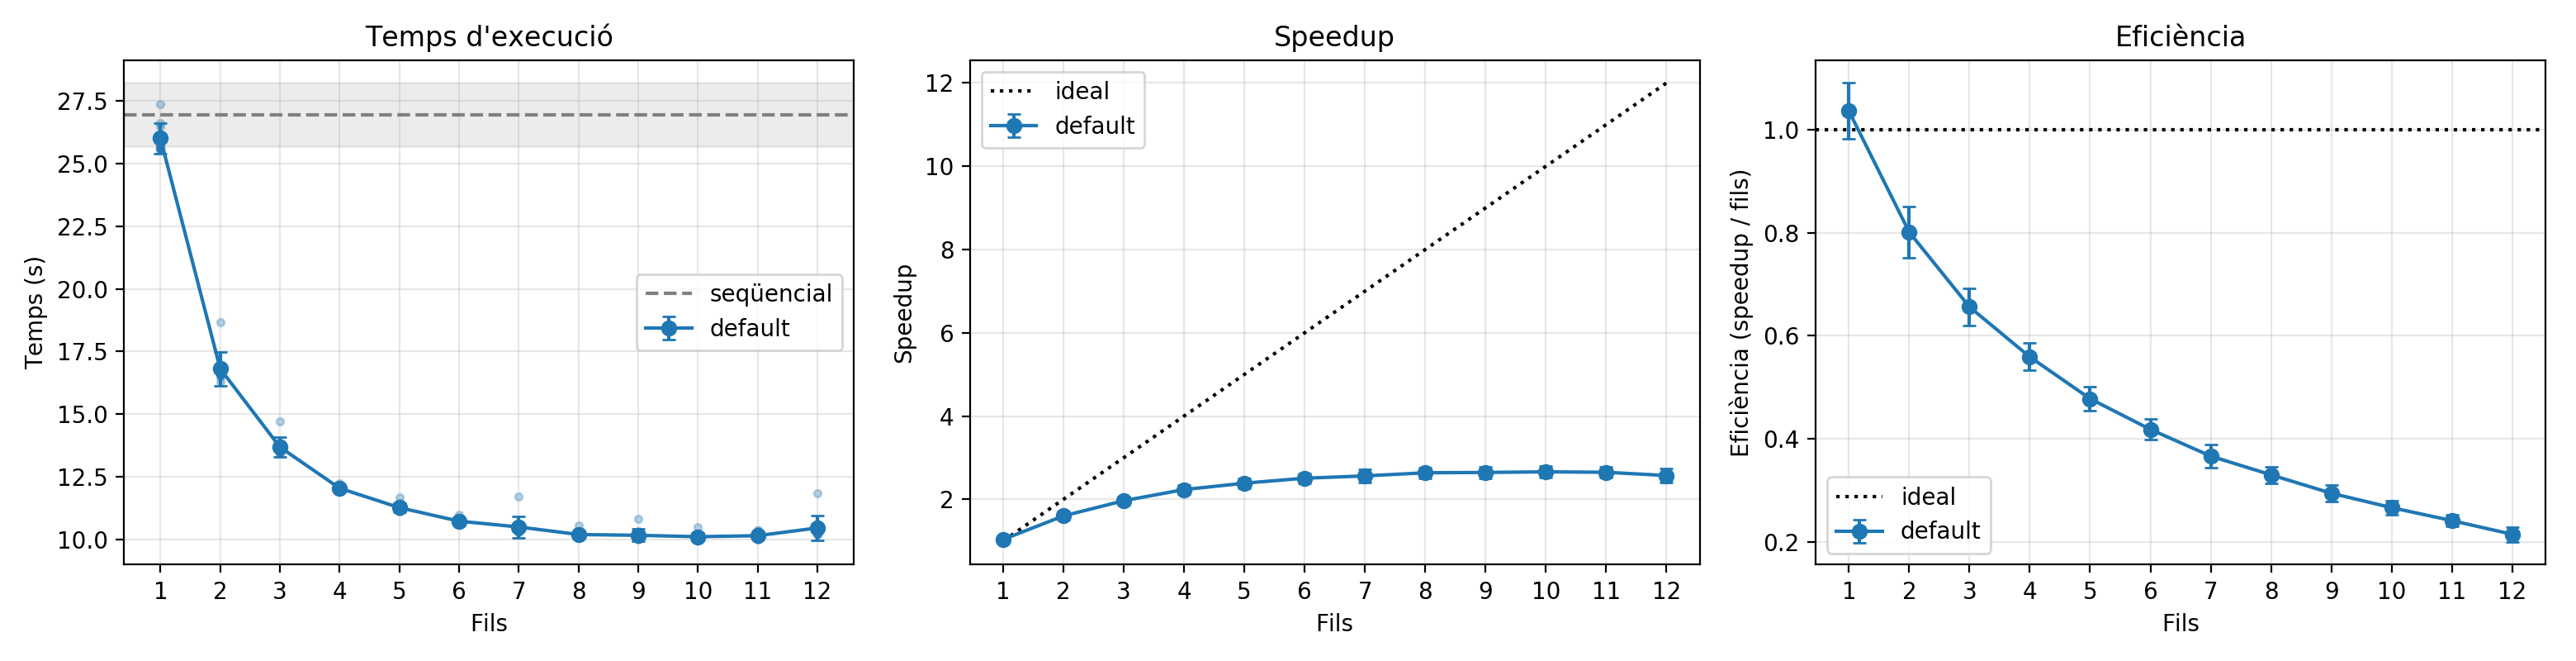
\includegraphics[width=1.7\textwidth]{Hidden_Part.png}
    }
    \caption{Comparació del temps d'execució, l'acceleració i l'eficiència segons el nombre de fils.}
    \label{fig:hidden_part}
\end{figure}

Ara es veu que aquesta paral·lelització sí aporta un gran benefici, amb una reducció substancial de temps i un \textit{speedup} creixient fins als $10$ threads.

També es pot comprovar en la taula percentual.
\begin{table}[H]
\centering
\begin{tabular}{|c|c|c|c|}
\hline
\textbf{Fils} & \textbf{Temps (s)} & \textbf{Diferència (s)} & \textbf{Diferència (\%)} \\ \hline
seq & 26,940 & 16,818 & 166,15 \\ \hline
1 & 25,996 & 15,874 & 156,83 \\ \hline
2 & 16,814 & 6,692 & 66,11 \\ \hline
3 & 13,693 & 3,571 & 35,28 \\ \hline
4 & 12,053 & 1,931 & 19,08 \\ \hline
5 & 11,280 & 1,158 & 11,44 \\ \hline
6 & 10,741 & 0,619 & 6,12 \\ \hline
7 & 10,510 & 0,388 & 3,83 \\ \hline
8 & 10,209 & 0,087 & 0,86 \\ \hline
9 & 10,177 & 0,055 & 0,54 \\ \hline
10 & 10,122 & 0,000 & 0,00 \\ \hline
11 & 10,162 & 0,040 & 0,40 \\ \hline
12 & 10,472 & 0,350 & 3,46 \\ \hline
\end{tabular}
\caption{Diferència del temps mitjà de cada configuració respecte al millor temps (10 fils, 10,122 s) amb la paral·lelització de les \textit{Output layers} i les \textit{Hidden layers} a \textit{back\_prop()}.}
\label{tab:dif_millor_bp_hid}
\end{table}

Finalment, queda estudiar si canviar la política de distribució de treball d'OpenMP pot ajudar o és contraproduent. S'usa la mateixa metodologia que a la funció \textit{forward\_prop()}, amb mides de \textbf{\texttt{chunk}} d'1, 2, 4, 8 i 16 per a \textbf{\texttt{dynamic}} i \textbf{\texttt{guided}}.

Es realitzen les execucions amb $10$ threads, ja que és el nombre de threads que ha resultat amb millor temps.

\begin{table}[H]
\centering
\begin{tabular}{|c|c|c|c|}
\hline
\textbf{Política} & \textbf{Chunk} & \textbf{Temps (s)} & \textbf{Dif. respecte \textit{static} (\%)} \\ \hline
\multirow{1}{*}{\textit{static}} & --- & \textbf{10,107 $\pm$ 0,071} & \textbf{0,00} \\ \hline
\multirow{5}{*}{\textit{dynamic}} & 1 & 20,126 $\pm$ 0,082 & 99,12 \\ \cline{2-4}
 & 2 & 16,897 $\pm$ 0,094 & 67,17 \\ \cline{2-4}
 & 4 & 14,931 $\pm$ 0,241 & 47,73 \\ \cline{2-4}
 & 8 & 13,451 $\pm$ 0,061 & 33,08 \\ \cline{2-4}
 & 16 & 12,983 $\pm$ 0,342 & 28,45 \\ \hline
\multirow{5}{*}{\textit{guided}} & 1 & 13,805 $\pm$ 0,164 & 36,59 \\ \cline{2-4}
 & 2 & 13,610 $\pm$ 0,156 & 34,65 \\ \cline{2-4}
 & 4 & 13,317 $\pm$ 0,095 & 31,76 \\ \cline{2-4}
 & 8 & 13,147 $\pm$ 0,130 & 30,07 \\ \cline{2-4}
 & 16 & 12,924 $\pm$ 0,080 & 27,87 \\ \hline
\end{tabular}
\caption{Temps d'execució segons la política i la mida de \textit{chunk} amb 10 fils (mitjana $\pm$ desviació estàndard).}
\label{tab:politiques2}
\end{table}

Les dades recollides en la taula ens podrien indicar que augmentar la mida del \textbf{\texttt{chunk}} podria ser beneficiós, i anar reduint el temps d'execució, però una comprovació amb \textbf{\texttt{chunk = 32}} ha descartat aquesta possibilitat.

\noindent Per tant, la millor política de distribució és \textbf{\texttt{schedule(static)}}, i el codi paral·lelitzat de la funció és el descrit anteriorment. Això es deu al fet que les operacions que duen a terme els threads tenen un cost computacional similar, és a dir, no hi ha una gran diferència en el temps d'execució de les diferents iteracions. Per tant, utilitzar una política de distribució dinàmica acaba introduint una sobrecàrrega addicional a l'hora de repartir les iteracions entre els threads, fet que pot augmentar el temps total d'execució.
 

\subsection{Fine-tuning global}

Queda decidir sobre els següents ítems:

\begin{itemize}
    \item Paral·lelitzar la funció \textit{feed\_input()}
    \item Paral·lelitzar la funció \textit{init\_deltas()}.
    \item Paral·lelitzar la funció \textit{update\_weights()}.
    \item Paral·lelitzar la funció \textit{compute\_loss()}.
\end{itemize}

És a dir, volem saber si les funcions que, paral·lelitzades per elles soles no aporten benefici, en conjunt sí que n'aporten.

Per comprovar-ho s'afegiran les funcions paral·lelitzades d'una en una sobre la base de \textbf{\texttt{training.c}} amb les funcions \textit{forward\_prop()} i \textit{back\_prop()} paral·lelitzades.

El temps des del que es parteix és el següent.

\begin{table}[H]
\centering
\begin{tabular}{|c|c|c|c|}
\hline
\textbf{Fils} & \textbf{Temps (s)} & \textbf{Speedup} & \textbf{Eficiència} \\ \hline
1 & 42,265 $\pm$ 0,671 & 1,00 $\pm$ 0,02 & 1,00 \\ \hline
2 & 22,250 $\pm$ 0,263 & 1,90 $\pm$ 0,04 & 0,95 \\ \hline
3 & 17,017 $\pm$ 0,544 & 2,48 $\pm$ 0,09 & 0,83 \\ \hline
4 & 13,316 $\pm$ 0,232 & 3,17 $\pm$ 0,07 & 0,79 \\ \hline
5 & 11,343 $\pm$ 0,119 & 3,73 $\pm$ 0,07 & 0,75 \\ \hline
6 & 10,329 $\pm$ 0,168 & 4,09 $\pm$ 0,09 & 0,68 \\ \hline
7 & 9,132 $\pm$ 0,047 & 4,63 $\pm$ 0,08 & 0,66 \\ \hline
8 & 8,373 $\pm$ 0,085 & 5,05 $\pm$ 0,10 & 0,63 \\ \hline
9 & 7,830 $\pm$ 0,039 & 5,40 $\pm$ 0,09 & 0,60 \\ \hline
10 & 7,521 $\pm$ 0,070 & 5,62 $\pm$ 0,10 & 0,56 \\ \hline
11 & 7,336 $\pm$ 0,091 & 5,76 $\pm$ 0,12 & 0,52 \\ \hline
12 & 8,115 $\pm$ 1,262 & 5,21 $\pm$ 0,81 & 0,43 \\ \hline
\end{tabular}
\caption{Mitjana $\pm$ desviació estàndard de les execucions amb les paral·lelitzacions ajustades de \textit{forward\_prop()} i \textit{back\_prop()}.  }
\label{tab:resultats4}
\end{table}

Es veu que la paral·lelització d'aquestes dues funcions ja aporta un gran benefici, si afegim la paral·lelització de la funció \textit{feed\_input()} obtenim els seguents temps.

\begin{table}[H]
\centering
\begin{tabular}{|c|c|c|c|}
\hline
\textbf{Fils} & \textbf{Temps (s)} & \textbf{Speedup} & \textbf{Eficiència} \\ \hline
1 & 40,635 $\pm$ 0,892 & 1,00 $\pm$ 0,03 & 1,00 \\ \hline
2 & 21,325 $\pm$ 0,143 & 1,91 $\pm$ 0,04 & 0,95 \\ \hline
3 & 14,836 $\pm$ 0,067 & 2,74 $\pm$ 0,06 & 0,91 \\ \hline
4 & 11,543 $\pm$ 0,072 & 3,52 $\pm$ 0,08 & 0,88 \\ \hline
5 & 9,688 $\pm$ 0,053 & 4,19 $\pm$ 0,09 & 0,84 \\ \hline
6 & 8,701 $\pm$ 0,047 & 4,67 $\pm$ 0,11 & 0,78 \\ \hline
7 & 7,768 $\pm$ 0,069 & 5,23 $\pm$ 0,12 & 0,75 \\ \hline
8 & 7,194 $\pm$ 0,043 & 5,65 $\pm$ 0,13 & 0,71 \\ \hline
9 & 6,762 $\pm$ 0,033 & 6,01 $\pm$ 0,14 & 0,67 \\ \hline
10 & 6,580 $\pm$ 0,032 & 6,18 $\pm$ 0,14 & 0,62 \\ \hline
11 & 6,466 $\pm$ 0,046 & 6,28 $\pm$ 0,15 & 0,57 \\ \hline
12 & 6,486 $\pm$ 0,076 & 6,26 $\pm$ 0,16 & 0,52 \\ \hline
\end{tabular}
\caption{Mitjana $\pm$ desviació estàndard de les execucions afegint la paral·lelització de \textit{feed\_input()}.}
\label{tab:resultats5}
\end{table}

En afegir aquesta funció s'obté una millora d'entre $1$ i $2$ segons al llarg de totes les execucions, i fins i tot, la variabilitat dels temps ha disminuït. Continuem afegint paral·lelitzacions i agregem la funció \textit{init\_deltas()}.

\begin{table}[H]
\centering
\begin{tabular}{|c|c|c|c|}
\hline
\textbf{Fils} & \textbf{Temps (s)} & \textbf{Speedup} & \textbf{Eficiència} \\ \hline
1 & 40,618 $\pm$ 0,726 & 1,00 $\pm$ 0,03 & 1,00 \\ \hline
2 & 20,683 $\pm$ 0,122 & 1,96 $\pm$ 0,04 & 0,98 \\ \hline
3 & 14,286 $\pm$ 0,055 & 2,84 $\pm$ 0,05 & 0,95 \\ \hline
4 & 11,095 $\pm$ 0,036 & 3,66 $\pm$ 0,07 & 0,92 \\ \hline
5 & 9,296 $\pm$ 0,044 & 4,37 $\pm$ 0,08 & 0,87 \\ \hline
6 & 8,316 $\pm$ 0,099 & 4,88 $\pm$ 0,11 & 0,81 \\ \hline
7 & 7,461 $\pm$ 0,083 & 5,44 $\pm$ 0,11 & 0,78 \\ \hline
8 & 6,971 $\pm$ 0,139 & 5,83 $\pm$ 0,16 & 0,73 \\ \hline
9 & 6,613 $\pm$ 0,072 & 6,14 $\pm$ 0,13 & 0,68 \\ \hline
10 & 6,365 $\pm$ 0,088 & 6,38 $\pm$ 0,14 & 0,64 \\ \hline
11 & 6,346 $\pm$ 0,138 & 6,40 $\pm$ 0,18 & 0,58 \\ \hline
12 & 6,487 $\pm$ 0,134 & 6,26 $\pm$ 0,17 & 0,52 \\ \hline
\end{tabular}
\caption{Mitjana $\pm$ desviació estàndard de les execucions afegint la paral·lelització de \textit{init\_deltas()}.}
\label{tab:resultats6}
\end{table}

S'ha continuat millorant el temps general, potser de manera no tant notòria en alguns dels casos, però segueix sent una addició positiva, per tant mantenim la funció paral·lelitzada i afegim la següent, \textit{compute\_loss()}.

\begin{table}[H]
\centering
\begin{tabular}{|c|c|c|c|}
\hline
\textbf{Fils} & \textbf{Temps (s)} & \textbf{Speedup} & \textbf{Eficiència} \\ \hline
1 & 40,809 $\pm$ 0,757 & 1,00 $\pm$ 0,03 & 1,00 \\ \hline
2 & 20,784 $\pm$ 0,055 & 1,96 $\pm$ 0,04 & 0,98 \\ \hline
3 & 14,366 $\pm$ 0,052 & 2,84 $\pm$ 0,05 & 0,95 \\ \hline
4 & 11,158 $\pm$ 0,045 & 3,66 $\pm$ 0,07 & 0,91 \\ \hline
5 & 9,353 $\pm$ 0,044 & 4,36 $\pm$ 0,08 & 0,87 \\ \hline
6 & 8,254 $\pm$ 0,065 & 4,94 $\pm$ 0,10 & 0,82 \\ \hline
7 & 7,424 $\pm$ 0,041 & 5,50 $\pm$ 0,11 & 0,79 \\ \hline
8 & 6,910 $\pm$ 0,043 & 5,91 $\pm$ 0,12 & 0,74 \\ \hline
9 & 6,571 $\pm$ 0,071 & 6,21 $\pm$ 0,13 & 0,69 \\ \hline
10 & 6,380 $\pm$ 0,030 & 6,40 $\pm$ 0,12 & 0,64 \\ \hline
11 & 6,259 $\pm$ 0,053 & 6,52 $\pm$ 0,13 & 0,59 \\ \hline
12 & 6,355 $\pm$ 0,193 & 6,42 $\pm$ 0,23 & 0,54 \\ \hline
\end{tabular}
\caption{Mitjana $\pm$ desviació estàndard de les execucions afegint la paral·lelització de \textit{compute\_loss()}.}
\label{tab:resultats7}
\end{table}

Aquí el benefici és quasi nul, millorant el temps  i el \textit{speedup} unes dècimes en les execucions amb alt nombre de threads. 
S'estudiarà si, en afegir l'ultima funció que resta per paral·lelitzar, la paral·lelització de la funció \textit{compute\_loss()} aporta un benefici o no. De moment es manté ja que no empitjora el programa.

La taula amb la funció \textit{update\_weights()} és la següent.

\begin{table}[H]
\centering
\begin{tabular}{|c|c|c|c|}
\hline
\textbf{Fils} & \textbf{Temps (s)} & \textbf{Speedup} & \textbf{Eficiència} \\ \hline
1 & 40,820 $\pm$ 0,853 & 1,00 $\pm$ 0,03 & 1,00 \\ \hline
2 & 20,403 $\pm$ 0,053 & 2,00 $\pm$ 0,04 & 1,00 \\ \hline
3 & 14,037 $\pm$ 0,115 & 2,91 $\pm$ 0,07 & 0,97 \\ \hline
4 & 10,716 $\pm$ 0,064 & 3,81 $\pm$ 0,08 & 0,95 \\ \hline
5 & 8,876 $\pm$ 0,031 & 4,60 $\pm$ 0,10 & 0,92 \\ \hline
6 & 7,748 $\pm$ 0,060 & 5,27 $\pm$ 0,12 & 0,88 \\ \hline
7 & 6,947 $\pm$ 0,038 & 5,88 $\pm$ 0,13 & 0,84 \\ \hline
8 & 6,423 $\pm$ 0,043 & 6,36 $\pm$ 0,14 & 0,79 \\ \hline
9 & 6,024 $\pm$ 0,056 & 6,78 $\pm$ 0,16 & 0,75 \\ \hline
10 & 5,824 $\pm$ 0,039 & 7,01 $\pm$ 0,15 & 0,70 \\ \hline
11 & 5,720 $\pm$ 0,044 & 7,14 $\pm$ 0,16 & 0,65 \\ \hline
12 & 5,757 $\pm$ 0,102 & 7,09 $\pm$ 0,19 & 0,59 \\ \hline
\end{tabular}
\caption{Mitjana $\pm$ desviació estàndard de les execucions afegint la paral·lelització de \textit{update\_weights()}.}
\label{tab:resultats8}
\end{table}

Amb aquesta última funció paral·lelitzada s'ha vist una millora d'uns $0,5s$ a partir de l'ús de $4$ threads, per tant es manté aquesta paral·lelització.

Finalment es comprova si traient la paral·lelització de la funció \textit{compute\_loss()} s'obté algun benefici, ja que s'ha vist que no aportava gran millora per si sola.

\begin{table}[H]
\centering
\begin{tabular}{|c|c|c|c|}
\hline
\textbf{Fils} & \textbf{Temps (s)} & \textbf{Speedup} & \textbf{Eficiència} \\ \hline
1 & 41,565 $\pm$ 2,008 & 1,00 $\pm$ 0,07 & 1,00 \\ \hline
2 & 20,620 $\pm$ 0,907 & 2,02 $\pm$ 0,13 & 1,01 \\ \hline
3 & 13,878 $\pm$ 0,040 & 3,00 $\pm$ 0,14 & 1,00 \\ \hline
4 & 10,903 $\pm$ 0,829 & 3,81 $\pm$ 0,34 & 0,95 \\ \hline
5 & 9,270 $\pm$ 0,900 & 4,48 $\pm$ 0,49 & 0,90 \\ \hline
6 & 8,092 $\pm$ 0,795 & 5,14 $\pm$ 0,56 & 0,86 \\ \hline
7 & 6,904 $\pm$ 0,026 & 6,02 $\pm$ 0,29 & 0,86 \\ \hline
8 & 6,338 $\pm$ 0,033 & 6,56 $\pm$ 0,32 & 0,82 \\ \hline
9 & 5,963 $\pm$ 0,102 & 6,97 $\pm$ 0,36 & 0,77 \\ \hline
10 & 5,936 $\pm$ 0,443 & 7,00 $\pm$ 0,62 & 0,70 \\ \hline
11 & 5,957 $\pm$ 0,501 & 6,98 $\pm$ 0,68 & 0,63 \\ \hline
12 & 5,690 $\pm$ 0,261 & 7,30 $\pm$ 0,49 & 0,61 \\ \hline
\end{tabular}
\caption{Mitjana $\pm$ desviació estàndard de les execucions traient la paral·lelització de \textit{compute\_loss()}.}
\label{tab:resultats9}
\end{table}

Donades aquestes dades, els temps mitjans són similars entre les dues versions i cap de les dues és més ràpida en totes les configuracions. No obstant això, en diverses execucions s'observa una menor desviació estàndard quan es manté la paral·lelització de \textit{compute\_loss()}. Per aquest motiu, s'ha decidit conservar-la.

\subsection{Comparació amb les dades de referència}

Un cop acabat l'ajust de paràmetres de paral·lelització, i amb una versió definitiva de totes les funcions paral·lelitzades, es compara el temps i l'\textit{speedup} de la nostra versió amb les dades de referència.

\begin{table}[H]
\centering
\begin{tabular}{|c|c|c|c|c|c|}
\hline
\textbf{Fils} & \textbf{Ref. (s)} & \textbf{Propi (s)} & \textbf{Dif. (s)} & \textbf{Dif. (\%)} & \textbf{Execs. $<$ ref.} \\ \hline
2 & 22,543 & 20,408 $\pm$ 0,044 & $-$2,135 & $-$9,47 & 20/20 \\ \hline
4 & 11,730 & 10,707 $\pm$ 0,036 & $-$1,023 & $-$8,72 & 20/20 \\ \hline
6 & 8,309 & 7,745 $\pm$ 0,034 & $-$0,564 & $-$6,79 & 20/20 \\ \hline
12 & 5,264 & 5,722 $\pm$ 0,135 & 0,458 & 8,71 & 0/20 \\ \hline
\end{tabular}
\caption{Comparació del temps d'execució propi (mitjana $\pm$ desviació estàndard de 20 execucions) amb el temps de referència. Els valors negatius indiquen un temps inferior al de referència.}
\label{tab:comp_temps}
\end{table}

\begin{table}[H]
\centering
\begin{tabular}{|c|c|c|c|c|}
\hline
\textbf{Fils} & \textbf{Speedup ref.} & \textbf{Speedup propi} & \textbf{Eficiència ref.} & \textbf{Eficiència pròpia} \\ \hline
2 & 1,81 & 2,00 $\pm$ 0,00 & 0,90 & 1,00 \\ \hline
4 & 3,47 & 3,80 $\pm$ 0,01 & 0,87 & 0,95 \\ \hline
6 & 4,90 & 5,26 $\pm$ 0,02 & 0,82 & 0,88 \\ \hline
12 & 7,74 & 7,12 $\pm$ 0,17 & 0,64 & 0,59 \\ \hline
\end{tabular}
\caption{Speedup i eficiència propis i de referència, calculats amb el temps seqüencial de referència (40,738 s).}
\label{tab:comp_speedup}
\end{table}

Com es pot veure a les taules, el codi paral·lelitzat que hem fet assoleix els temps de referència en els casos de $2, 4$ i $6$ threads, però es queda enrere en el cas de $12$ threads. El mateix passa amb el \textit{speedup} i l'eficiència. 

Tot i això, no està gaire lluny dels paràmetres de referència l'execució amb $12$ threads, amb una diferència de $0,458 \pm 0,135s$ en el temps, $0,62 \pm 0,17$ d'\textit{speedup} i $0,05$ punts en l'eficiència.

Respecte als encerts, s'han mantingut estables al llarg de tota la pràctica, excepte en els punts comentats a la secció \texttt{\nameref{sec:error_spike}}. Les dades d'aquestes últimes execucions han sigut les següents:

\begin{itemize}
    \item 923 (/946): 1 execució.
    \item 927 (/946): 5 execucions.
    \item 928 (/946): 24 execucions.
    \item 929 (/946): 46 execucions.
    \item 930 (/946): 4 execucions.
\end{itemize}



\newpage
\section{Problemes trobats}

\subsection{Concepte de SIMD}
\label{sec:simd_explanation}

\textbf{SIMD} és un acrònim que significa \textit{Single instruction, multiple data}, i la directiva d'OpenMP \textbf{\#pragma omp simd} serveix per executar diverses iteracions d'un bucle simultàniament mitjançant instruccions \textbf{SIMD} del processador.

L'avantatge de \textbf{SIMD} és que, en lloc de gestionar i executar les operacions de suma i producte individualment per a cada iteració, el processador pot treballar amb grups d'elements mitjançant instruccions vectorials. La mida dels grups depèn del processador, concretament de l'arquitectura d'aquest, i de la mida de les dades.

\subsection{Baixada d'encerts sense la directiva \textbf{\texttt{\#pragma omp single}} (Condició de carrera)}
\label{sec:error_spike}


\noindent En fer la paral·lelització bàsica, ens vam trobar amb una reducció molt gran del nombre d'encerts a causa de les condicions de carrera que es produïen entre els threads en els dobles bucles de la funció. Inicialment, com que havíem paral·lelitzat les altres parts però no havíem afegit explícitament la directiva \textbf{\texttt{\#pragma omp for}} en aquests bucles, pensàvem que només els executaria un thread.

\bigskip

\noindent Finalment, vam observar que, en trobar-se dins d'una regió \textbf{\texttt{\#pragma omp parallel}}, tots els threads executaven íntegrament aquests bucles, en lloc de repartir-se'n les iteracions. Això provocava que diversos threads realitzessin els mateixos càlculs i modifiquessin simultàniament les mateixes posicions dels vectors \textbf{\texttt{dw}} i \textbf{\texttt{dactv}}, generant condicions de carrera en les operacions d'acumulació. Com a conseqüència, el càlcul dels gradients podia ser incorrecte, fet que explicava la gran disminució del nombre d'encerts.

\bigskip

\noindent Això ens va portar a utilitzar la directiva \textbf{\texttt{\#pragma omp single}}, que fa que el bucle sigui executat per un únic thread, com si es tractés d'una execució seqüencial. D'aquesta manera, aconseguim evitar les condicions de carrera i la repetició dels càlculs, recuperant el nombre d'encerts correcte. No obstant això, el temps d'execució d'aquesta part no havia de ser necessàriament igual al de la versió seqüencial, a causa de la sobrecàrrega associada a la gestió dels threads i a la sincronització dins de la regió paral·lela.



\subsection{Augment del temps d'execució a causa de l'ús de la directiva \textbf{\texttt{\#pragma omp atomic}}}
\label{sec:error_spike2}


\noindent Una alternativa per evitar les condicions de carrera en paral·lelitzar els dobles bucles de la funció \textbf{\texttt{back\_prop()}} era utilitzar la directiva \textbf{\texttt{\#pragma omp atomic}}. Aquesta permet que diversos threads executin el bucle simultàniament, garantint que les actualitzacions sobre una mateixa posició de memòria es realitzin de manera atòmica. No obstant això, aquesta sincronització pot incrementar considerablement el temps d'execució quan diferents threads intenten modificar repetidament els mateixos elements del vector \textbf{\texttt{dactv}}.

\bigskip

\noindent En el nostre cas, aquest problema es produïa perquè paral·lelitzàvem el bucle d'índex $j$, mentre que cada thread recorria els mateixos valors de $k$, de manera que diversos threads podien intentar acumular simultàniament les seves contribucions sobre una mateixa posició de \textbf{\texttt{dactv[k]}}. Aquest fet era especialment rellevant a les \textit{Hidden Layers}, on els dobles bucles realitzen un total de 645.350 iteracions, corresponents a les combinacions de neurones de les capes 3, 2 i 1 amb les seves capes anteriors. D'aquestes, 133.350 requereixen una acumulació sobre \textbf{\texttt{dactv}}, cosa que implicava executar el mateix nombre d'operacions atòmiques per cada crida a \textbf{\texttt{back\_prop()}}. Com que aquesta funció s'executa repetidament durant l'entrenament, la sobrecàrrega associada a aquestes sincronitzacions podia acabar afectant significativament el temps total d'execució.

\bigskip

\noindent Per aquest motiu, es va considerar substituir la directiva \textbf{\texttt{\#pragma omp atomic}} per la clàusula \textbf{\texttt{reduction}}. Aquesta alternativa permet que cada thread acumuli les seves contribucions en una còpia privada del vector \textbf{\texttt{dactv}}, evitant la necessitat de sincronitzar individualment cada suma. Un cop finalitzat el bucle, OpenMP s'encarrega de combinar les contribucions de les còpies privades sobre el vector original. D'aquesta manera, es busca reduir la sobrecàrrega de sincronització i millorar el rendiment de la paral·lelització, tot i que la reducció també comporta un cost associat a la creació i combinació dels vectors privats.

\newpage
\section{Conclusions}

\noindent En aquesta pràctica hem treballat en la paral·lelització d'un programa en C que implementa una xarxa neuronal, amb l'objectiu de reduir-ne el temps d'execució mitjançant OpenMP. Per aconseguir-ho, hem analitzat les diferents funcions del programa i hem estudiat quines parts es podien paral·lelitzar, tenint en compte els possibles problemes que podien aparèixer i les diferents alternatives per solucionar-los.

\bigskip

\noindent Els resultats han mostrat que no totes les funcions es beneficien de la paral·lelització individualment, especialment quan presenten poca càrrega computacional i la sobrecàrrega de gestió dels threads és comparable al treball realitzat. En canvi, les funcions \texttt{forward\_prop()} i \texttt{back\_prop()} han estat especialment rellevants per aconseguir una reducció del temps total d'execució.

\bigskip

\noindent Durant el procés d'optimització, s'han identificat diferents problemes relacionats amb les condicions de carrera, les dependències entre iteracions i el cost de les operacions atòmiques. L'ús de reduccions ha permès paral·lelitzar acumulacions compartides que inicialment s'havien executat de manera seqüencial mitjançant la directiva \textbf{\texttt{\#pragma omp single}}.

\bigskip

\noindent Pel que fa al rendiment, la versió final ha obtingut uns temps mitjans de 20,408 s, 10,707 s, 7,745 s i 5,722 s amb 2, 4, 6 i 12 threads, respectivament. En comparació amb els temps proporcionats com a referència, s'han aconseguit millores amb 2, 4 i 6 threads, mentre que amb 12 threads el temps ha estat lleugerament superior.

\bigskip

\noindent Finalment, aquesta pràctica ha permès comprovar que una paral·lelització eficient no consisteix únicament a distribuir iteracions entre threads, sinó també a gestionar adequadament les dependències, reduir la sobrecàrrega de sincronització i escollir una distribució del treball apropiada per a cada situació.


\newpage
\section{Ús de IA}

En aquesta pràctica s'ha fet ús d'Intel·ligència artificial per diverses tasques, amb el motiu de l'aclariment de conceptes, correcció d'errors tipogràfics i conceptuals i automatització de tasques repetitives.

S'han usat scripts de Python generats per IA que recollien les dades generades en els \texttt{slurm-*.out} i generaven les taules i els gràfics presentats en aquest informe, ja que representava una tasca repetitiva amb càlculs de mitjanes i variàncies que no representen cap complicació conceptual.

També s'ha usat la IA per fer recerca de conceptes, com el concepte de \textbf{SIMD} explicat anteriorment. La IA ha sigut una de les eines de recerca, s'ha complementat l'informació amb altres fonts, esmentades en la bibliografia.

\newpage
\nocite{wiki_simd, openmp_refguides}   % o \nocite{*} per incloure-hi totes les entrades del .bib
\bibliographystyle{IEEEtran}
\bibliography{references}
\end{document}
